
\clearpage
\section{La gestion de séances}

La fonction 'Gestion de séances' dans CUBE PA vous permet de :

% Probleme aufgetreten von hier bis (Probleme aufgetreten bis da) 5.5.2016

\begin{itemize}
\item
créer et envoyer une invitation à une séance
\item
créer et envoyer les procès-verbaux des séances
\item
créer et suivre des affaires en suspens
\item
documenter des décisions
\item
chercher et lire / modifier les invitations aux séances, les procès-verbaux, les affaires en suspens et les décisions
\end{itemize}

\vspace{2cm}

\begin{wrapfigure}[2]{l}{6.5cm}   % [x] Wie manche Zeile soll sich um die Grafik "brechen"
  \vspace{-35pt}      % Grundwert war 20; mit 30 schön oben beim Text ausgerichtet
  \begin{center}
    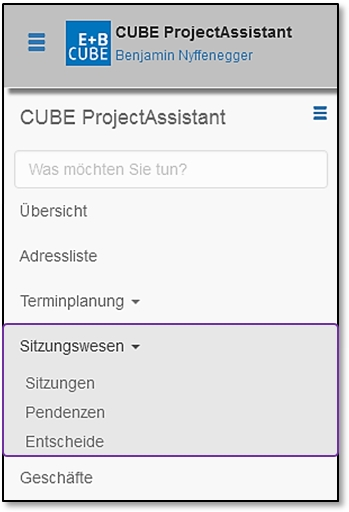
\includegraphics[width=1\linewidth]{../chapters/05_Sitzungswesen/pictures/5-1_Menu_Sitzungswesen.jpg}
  \end{center}
  \vspace{-20pt}
  \caption{Utiliser la gestion de séances}
  \vspace{-10pt}
\end{wrapfigure}

Dans le menu principal à gauche, choisissez d'abord l'élément 'Gestion de séances' puis le sous-élément 'Séances'.

\vspace{5cm}

\pagebreak
\textbf{L'aperçu des séances en bref :}

\begin{figure}[H]
\center{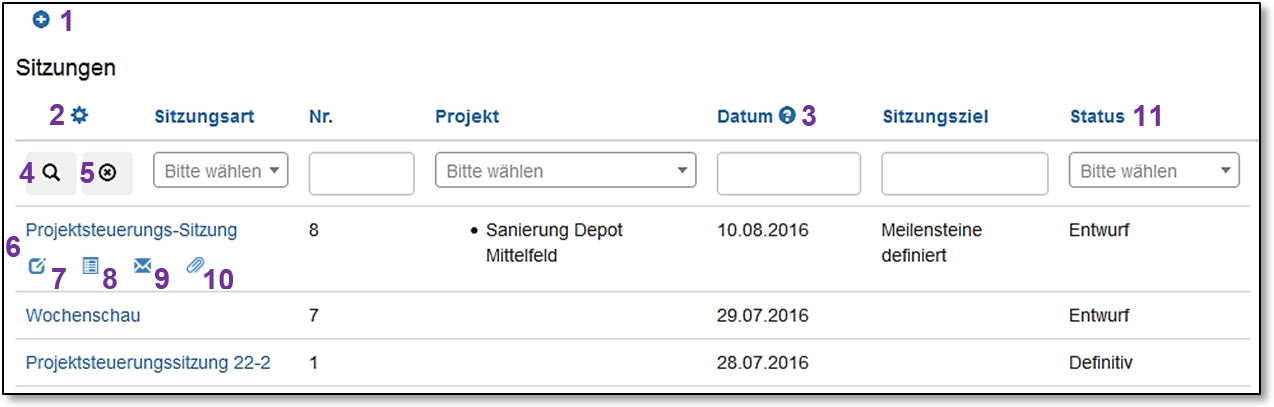
\includegraphics[width=1\linewidth]{../chapters/05_Sitzungswesen/pictures/5_SitzungenUebersicht.jpg}}
\caption{L'aperçu des séances}
% \label{fig:speciation}
\end{figure}

L'aperçu des séances comporte une vue des séances actuelles ou passées. Vous pouvez ajouter une nouvelle séance en cliquant le symbole plus 
\includegraphics[height=12pt]{/Icons/Plussymbol.jpg} \col{(1)}. Si vous trouvez que trop de colonnes sont affichées, vous pouvez en masquer quelques unes en cliquant le symbole de configuration 
\includegraphics[height=12pt]{/Icons/SpaltenEinst.jpg} \col{(2)}. Le point d'interrogation 
\includegraphics[height=12pt]{/Icons/Fragezeichen.jpg} \col{(3)} donne des informations sur les formats de dates ou les possibilités de recherche : 

\begin{figure}[H]
\center{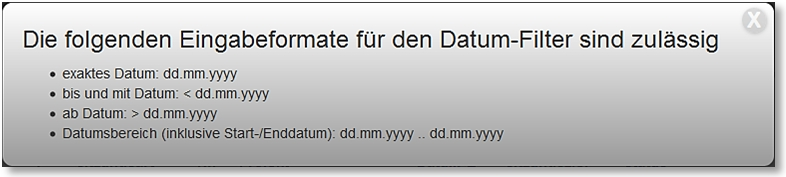
\includegraphics[width=0.7\linewidth]{../chapters/05_Sitzungswesen/pictures/5_Datumformat.jpg}}
% \caption{Das Menü in CUBE PA}
% \label{fig:speciation}
\end{figure}

Vous pouvez rechercher parmi les séance en utilisant le filtre. Saisissez des mots-clé ou choisissez une donnée du menu déroulant (par exemple projets). Après avoir défini le filtre, cliquez sur la loupe 
\includegraphics[height=12pt]{/Icons/Lupe_s.jpg} \col{(4)}. Toutes les données correspondant aux critères définis seront affichées. Cliquez sur la petite croix 
\includegraphics[height=12pt]{/Icons/FilterLoeschen.jpg} \col{(5)} pour effacer les critères de recherche du filtre. \\
Cliquez sur l'en-tête d'une colonne pour trier les résultats (par ordre croissant ou décroissant) selon cette colonne.

Si vous cliquez sur le titre d'une séance (en bleu), des options s'affichent \col{(6)} : Vous pouvez 

\begin{compactitem}
\item modifier une invitation à une séance 
\includegraphics[height=12pt]{/Icons/bearbeiten.jpg} \col{(7)},
\item importer l'invitation à la séance dans votre calendrier Outlook en tant que fichier .ics 
\includegraphics[height=12pt]{/Icons/Kalenderimport.jpg} \col{(8)},
\item modifier le procès-verbal de la séance 
\includegraphics[height=12pt]{/Icons/Listensymbol.jpg} \col{(9)},
\item envoyer l'invitation à la séance avec ses pièces jointes par e-mail 
\includegraphics[height=12pt]{/Icons/Versandsymbol.jpg} \col{(10)},
\item ouvrir ou sauvegarder l'invitation à la séance en tant que fichier PDF 
\includegraphics[height=12pt]{/Icons/Briefsymbol.jpg} \col{(11)} ou 
\item si l'invitation contient une pièce jointe, télécharger la pièce jointe en cliquant le symbole trombone 
\includegraphics[height=12pt]{/Icons/Bueroklammer.jpg} \col{(10)}.
\item copier une séance \col{(13)}. Plus d'informations au chapitre \ref{bkm:Ref2017112701}.
\end{compactitem}
	
La colonne 'Etat' \col{(14)} vous montre si le procès-verbal d'une séance a été archivé et est ainsi 'final'. Si la séance a cet état, les options mentionnées ne seront plus disponibles. Le symbole de feuille 
\includegraphics[height=12pt]{/Icons/Blattsymbol.jpg} s'affiche et vous permet d'ouvrir ou de sauvegarder le procès-verbal de la séance sous format PDF.
	
\vspace{\baselineskip}
\label{bkm:Ref2017112701}

\textbf{Copier une séance :} Cliquer sur le symbole 'copier' 
\includegraphics[height=12pt]{/Icons/kopieren.jpg} \col{(13)} pour dupliquer une séance existante. La fenêtre suivante s'ouvre : 

\begin{figure}[H]
\center{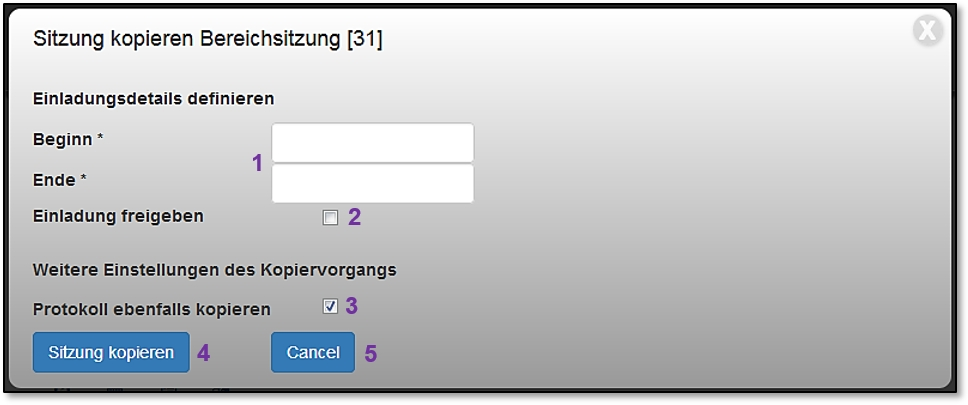
\includegraphics[width=1\linewidth]{../chapters/05_Sitzungswesen/pictures/5_SitzungKopieren.jpg}}
\caption{Copier une séance}
% \label{fig:speciation}
\end{figure}

Saisissez la nouvelle date et les temps de début et de fin de la copie \col{(1)}. Choisissez si l'invitation à la nouvelle séance est validée \col{(2)}. Vous pouvez également choisir d'inclure ou pas le protocole de la séance de base \col{(3)}. Cliquez ensuite sur 'Dupliquer la séance' \col{(4)} ou arrêter le processus en cliquant 'Annuler' \col{(5)}.

\vspace{\baselineskip}



\subsection{Invitation à une nouvelle séance}
\label{bkm:Ref434828480}

Cliquez sur le signe plus (ajouter) 
\includegraphics[height=12pt]{/Icons/Plussymbol.jpg} \col{(1)} en haut à gauche.

\vspace{\baselineskip}

\begin{figure}[H]
\center{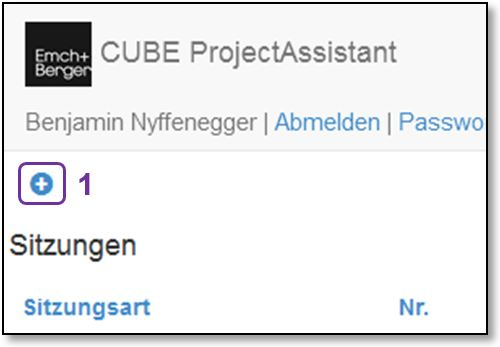
\includegraphics[width=0.4\linewidth]{51_Neue_Sitzung.jpg}}
\caption{Ajouter une nouvelle séance}
% \label{fig:speciation}
\end{figure}

% \vspace{\baselineskip}

Le masque pour saisir une nouvelle séance s'affiche :

\begin{figure}[H]
\center{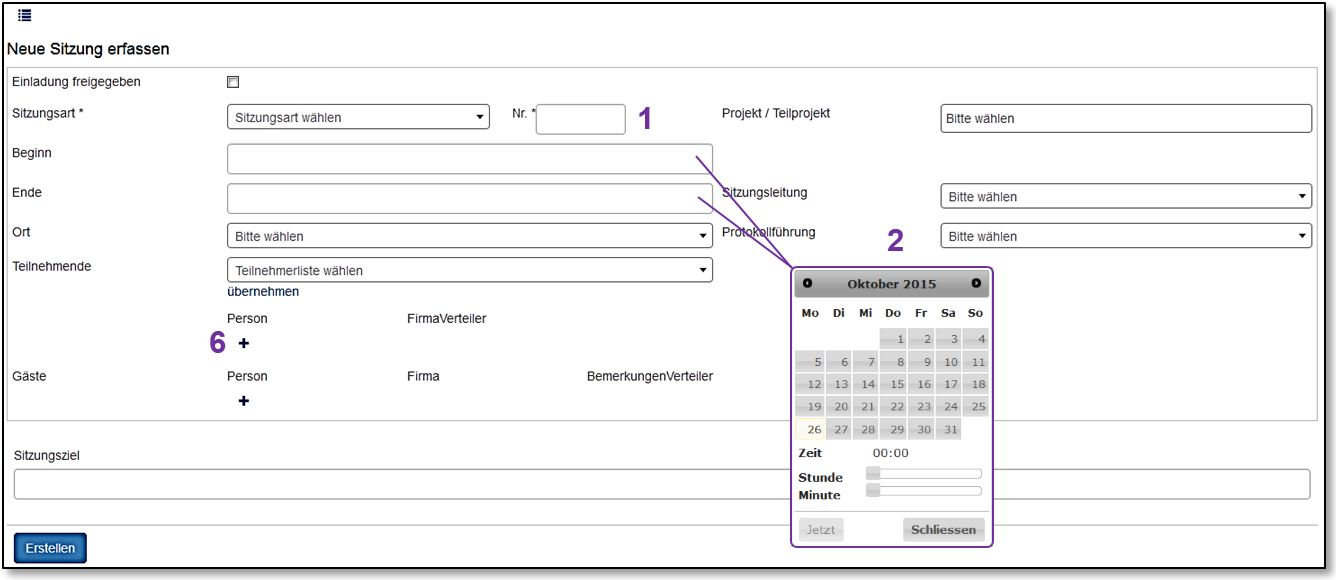
\includegraphics[width=1\linewidth]{51_Neue_Sitzung_erfassen.jpg}}
\caption{Saisir une nouvelle séance}
% \label{fig:speciation}
\end{figure}

\begin{figure}[H]
\center{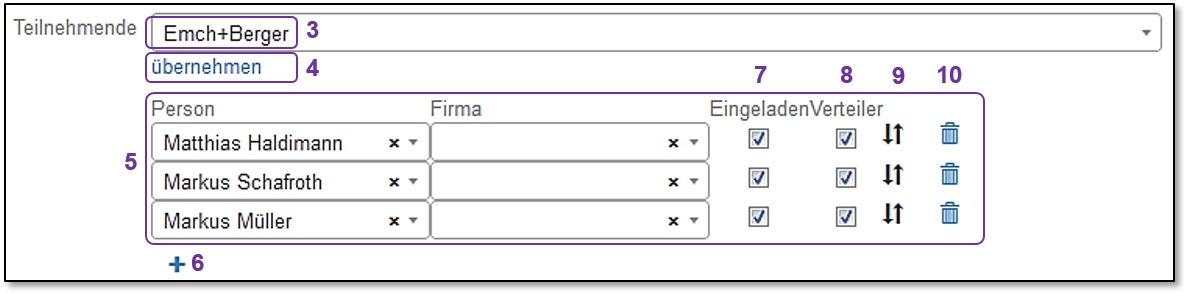
\includegraphics[width=1\linewidth]{../chapters/05_Sitzungswesen/pictures/5-1_Neue_Sitzung_Teilnehmende.jpg}}
\caption{Inviter des participants à la séance}
% \label{fig:speciation}
\end{figure}

Remplissez le masque. Les champs obligatoires sont marqués avec un astérisque (*). Les points suivants sont les plus importants :

\begin{itemize}
\item 
Lorsque vous choisissez le type de séance, CUBE PA fixe automatiquement le numéro correspondant à la séance \col{(1)}.
\item 
Quand vous cliquez sur les champs 'Début' et 'Fin', un calendrier s'affiche et vous pouvez y définir la date et l'heure \col{(2)}. \textit{Quand vous saisissez le temps de début pour une séance, le temps de fin est automatiquement fixé à 30 minutes après le début.}
\item 
Pour le champ 'Participants' vous pouvez choisir une liste de participants prédéfinie \col{(3)} qui contient tous les participants usuels. Cliquez ensuite sur 'Actualiser' \col{(4)} et la liste de tous les participants s'affiche juste en-dessous \col{(5)}.
\item 
Si un participant supplémentaire qui ne fait pas partie de la liste prédéfinie doit être ajouté, ou  si vous voulez ajouter les participants ad hoc, cliquez sur le signe plus (ajouter) sous le champ 'Participants' \col{(6)} et choisissez les données correspondantes dans les champs 'Personne' et 'Entreprise'. 
\item
Vous pouvez choisir, pour chaque participant, s'il est invité à la séance ou s'il est uniquement sur la liste de distribution. Cochez la case \col{(7)} sous 'Invité', et plus tard dans le procès-verbal de séance, vous pouvez préciser si le participant était présent à la séance ou pas. Cochez la case sous 'Distribution' si le participant doit seulement apparaître dur la liste de distribution \col{(8)}.
\item 
Pour modifier l'ordre des participants, appuyez sur le symbole des deux flèches verticales 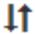
\includegraphics[height=12pt]{/Icons/VertPfeile.jpg} \col{(9)} près d'une saisie pour la glisser-déposer à la bonne position.
\item 
Cliquez sur la poubelle 
\includegraphics[height=12pt]{/Icons/Muelltonne.jpg} \col{(10)} pour supprimer un participant. Confirmez l'avertissement 'Enlever ?' en cliquant 'OK'.
\item 
Si un invité doit participer à la séance, par exemple pour un point spécifique de l'ordre du jour, vous pouvez l'ajouter en cliquant sur la signe plus (ajouter) dans le domaine 'Invités' et en saisissant les données correspondantes dans les champs 'Personne' et 'Entreprise'. Les autres symboles ont les mêmes fonctionnalités que ceux de du domaine 'Participants'.
\item 
Si une personne qui n'est pas dans les liste de sélections mentionnées plus haut (participants et invités) doit participer à la séance, vous devez d'abord l'ajouter dans la 'Gestion d'utilisateurs' (voir plus tard au chapitre \ref{bkm:Ref434828324}). Si une personne manque à une liste de participants prédéfinie, vous pouvez l'ajouter à la liste via l'élément de menu 'Configuration' puis le sous-élément 'Liste de participants à la séance', à condition que cette personne ait déjà été ajoutée dans la 'Gestion d'utilisateurs'.
\end{itemize}

Quand vous aurez saisi toutes les données, cliquez sur le bouton 'Créer' 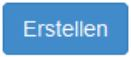
\includegraphics[height=12pt]{/Icons/B_Erstellen.jpg} en bas à gauche. Des champs additionnels s'affichent.

\begin{figure}[H]
\center{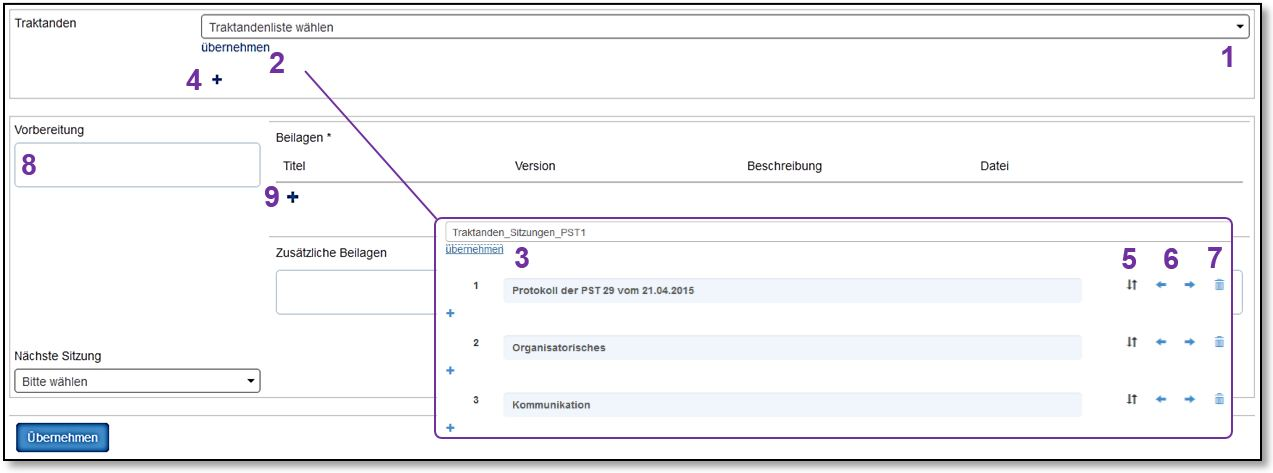
\includegraphics[width=1\linewidth]{51_Traktanden.jpg}}
\caption{Ajouter des points à l'ordre du jour}
% \label{fig:speciation}
\end{figure}

Les points suivants sont importants :

\begin{itemize}
\item 
Dans le champ 'Points d'ordre du jour' vous pouvez choisir une liste prédéfinie \col{(1)}, puis cliquer sur 'Actualiser' \col{(2)}. La liste de points d'ordre du jour est alors affichée \col{(3)}. Comme avec les participants, vous pouvez ajouter des points d'ordre du jour additionnels sous forme de texte libre en cliquant sur le signe plus (ajouter) \col{(4)} et modifier l'ordre des points en utilisant le symbole des flèches verticales \col{(5)}. Le symbole des flèches horizontales \col{(6)} vous permets de placer un point plus haut ou plus bas dans la hiérarchie de numération. Si un point de l'ordre du jour doit être supprimé, cliquez sur le symbole de poubelle 
\includegraphics[height=12pt]{/Icons/Muelltonne.jpg} \col{(7)} et confirmez l'avertissement de sécurité.
\item 
Dans la champ 'Préparation' vous pouvez saisir des informations sous forme de texte libre \col{(8)}. On entend par 'Préparation' les activités qui doivent être réalisées en avance pour un bon déroulement de la séance, par exemple préparer une présentation.
\end{itemize}

\textbf{Charger ou établir des liens à des pièces jointes:}
Vous pouvez charger des documents comme pièces jointes à un procès-verbal de séance. De plus, vous pouvez directement établir un lien à un document qui se trouve déjà dans le classement de documents de CUBE PA.  

\vspace{\baselineskip}

\begin{figure}[H]
\center{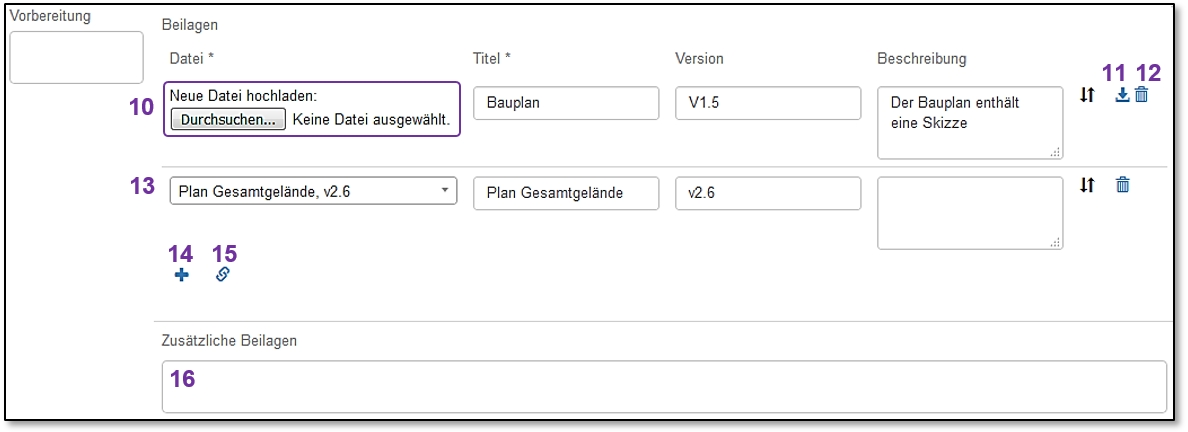
\includegraphics[width=1\linewidth]{../chapters/05_Sitzungswesen/pictures/5-1_BeilagenHochladenVerknuepfen.jpg}}
\caption{Charger ou établir des liens à des pièces jointes}
% \label{fig:speciation}
\end{figure}

\vspace{\baselineskip}

\begin{itemize}
\item 
Pour ajouter des pièces jointes à l'invitation à la séance, cliquez le signe plus (ajouter) sous 'Pièces Jointes' \col{(9)}. Vous pouvez saisir le titre, la version et la description de la pièce jointe. Sous 'Charger nouveau fichier' \col{(10)}, cliquez 'Naviguer' et choisissez la pièce jointe désirée puis cliquez 'Ouvrir'. La pièce jointe s'affichera dans l'aperçu personnel de chaque participant qui utilise CUBE PA. Le symbole de téléchargement \includegraphics[height=12pt]{/Icons/download.jpg} \col{(11)} vous permet de télécharger et de sauvegarder une pièce jointe. Vous pouvez changer l'ordre des pièces jointes par glisser-déposer en utilisant le symbole des flèches verticales ou supprimer une pièce jointe en cliquant sur le symbole de poubelle 
\includegraphics[height=12pt]{/Icons/Muelltonne.jpg}. Après l'avoir chargé, le fichier ou son nom devient visible :
\end{itemize}

\begin{figure}[H]
\center{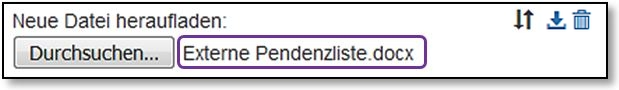
\includegraphics[width=0.5\linewidth]{../chapters/05_Sitzungswesen/pictures/5-1_NeueDateiHochladen.jpg}}
\caption{Le fichier chargé est visible}
% \label{fig:speciation}
\end{figure}

\textbf{Astuce :} Au lieu de cliquer sur 'Naviguer' pour choisir le document, vous pouvez glisser-déposer le document directement sur le champ 'Naviguer'. Le fichier sera chargé et lié à l'invitation à la séance.

\vspace{\baselineskip}

\begin{itemize}
\item
En outre de charger une pièce jointe, vous pouvez établir un lien depuis l'invitation ou le procès-verbal de la séance vers un document déjà chargé dans CUBE PA. Pour ce faire, cliquez sur le symbole de lien 
\includegraphics[height=12pt]{/Icons/Link.jpg} \col{(15)}. Sélectionnez la pièce jointe désirée sous 'Fichier' \col{(13)}. Vous pouvez optionnellement saisir un titre, une version, et une description. Utilisez le symbole des flèches verticales 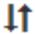
\includegraphics[height=12pt]{/Icons/VertPfeile.jpg} pour modifier l'ordre des pièces jointes.
\end{itemize}

\begin{itemize}
\item 
Pièces jointes supplémentaires \col{(16)} : Dans cette section, des pièces jointes supplémentaires qui n'ont pas été chargées sur CUBE PA et qui ne sont donc pas disponibles (par exemple des plans sous forme papier) peuvent être mentionnés.
\item 
Dans le champ 'Séance de suivi' vous pouvez simplement choisir la prochaine séance et elle va être affichée dans l'invitation avec son lieu et sa date. Ceci n'est possible que si l'invitation pour cette prochaine séance a déjà été créée.
\end{itemize}

Ayant rempli tous les champs, cliquez sur le bouton 'Actualiser'. 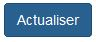
\includegraphics[height=12pt]{/Icons/B_Uebernehmen.jpg} \newline
Cliquez sur le symbole de lettre 
\includegraphics[height=12pt]{/Icons/Briefsymbol.jpg} en haut de la page à gauche. Ensuite l'invitation prête est affichée sous format PDF. Vous pouvez maintenant la sauvegarder sur votre ordinateur et l'envoyer aux participants par e-mail ou par poste.

\vspace{\baselineskip}

Partager l'invitation sur l'aperçu personnel :

\begin{itemize}
\item
Afin de partager l'invitation à la séance avec sa liste d'affaires en suspens et éventuelles pièces jointes sur l'aperçu personnel des invités, la case correspondante ('Invitation envoyée') doit être cochée :
\end{itemize}

\begin{figure}[H]
\center{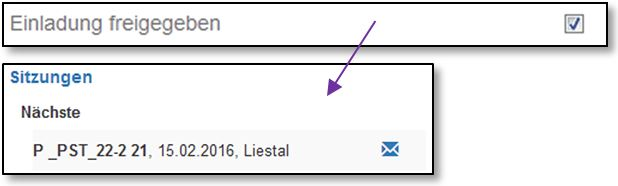
\includegraphics[width=0.5\linewidth]{51_EinladungFreigeben.jpg}}
\caption{Partager l'invitation}
% \label{fig:speciation}
\end{figure}

\begin{small}
La case 'Invitation envoyée' a été cochée en créant l'invitation à la séance. Le symbole de lettre est ainsi visible dans l'aperçu personnel.
\end{small}

\begin{itemize}
\item
Si la case n'est pas cochée, la date et le lieu de la séance sont affichés pour les utilisateurs, mais la liste des affaires en suspens et les pièces jointes ne sont pas disponibles pour télécharger.
\end{itemize}

\begin{figure}[H]
\center{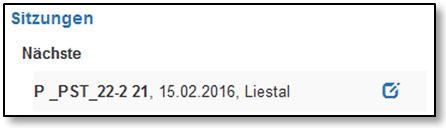
\includegraphics[width=0.5\linewidth]{51_SitzungenBearbeiten.jpg}}
\caption{Modifier une invitation à une séance}
% \label{fig:speciation}
\end{figure}

\begin{small}
La case 'Invitation envoyée' n'a pas été cochée en créant l'invitation à la séance. L'invitation à la séance peut être modifiée en cliquant le symbole d'édition dans l'aperçu personnel.
\end{small}

% Probleme aufgetreten bis da (Code könnte genommen werden von: 20160505_1724_LaTeX Document (neu)V2
% scheint, aber gut zu sein 5.5.2016, bny
% alle \liststyle etc... gelöscht Fehler von 143 auf 89 reduziert.

\subsection{Créer un procès-verbal}

Il existe deux possibilités pour enregistre un procès-verbal de séance dans CUBE PA :

\begin{enumerate}
\item
Vous pouvez saisir le procès-verbal directement dans CUBE PA. Ceci nécessite une connexion Internet qui fonctionne et est surtout recommandé si tous les participants utilisent CUBE PA, et l'utilisent aussi pour faire des commentaires dans les procès-verbaux de séances.
Il est aussi possible de prendre des notes simples durant la séance et de saisir le procès-verbal plus tard dans CUBE PA.
\item
Vous pouvez rédiger le procès-verbal dans un document hors CUBE PA et le charger ensuite sur CUBE PA, une fois approuvé.
Ceci est pratique si la séance ne suit pas les points d'ordre du jour définis dans l'invitation, si la séance n'est pas structurée, ou si beaucoup de participants n'utilisent pas CUBE PA.
\end{enumerate}

Pour certains projets il est important d'avoir une vision claire de qui a effectué des modifications dans les procès-verbaux de séances. CUBE PA dispose d'un mode d'édition avec suivi de modifications, mais l'utilisation de ce mode est facultative, comme celle du mode d'édition Microsoft Word.
Finalement c'est aux utilisateurs de surveiller les changements.

\subsubsection{Saisir un procès-verbal dans CUBE PA}

Une fois dans la salle de réunion, vérifiez que vous avez une connexion Internet et que vous êtes connectés au CUBE PA. Le symbole de connexion en bas à droite ne doit pas être rouge.

\vspace{\baselineskip}

Dans le menu principal à gauche, choisissez l'élément de menu 'Gestion de séances', puis le sous-élément 'Séances'. Vous êtes dirigé vers un aperçu de toutes les séances enregistrées dans CUBE PA, c'est-à-dire les séances pour lesquelles au moins une invitation a été créée. 

\begin{figure}[H]
\center{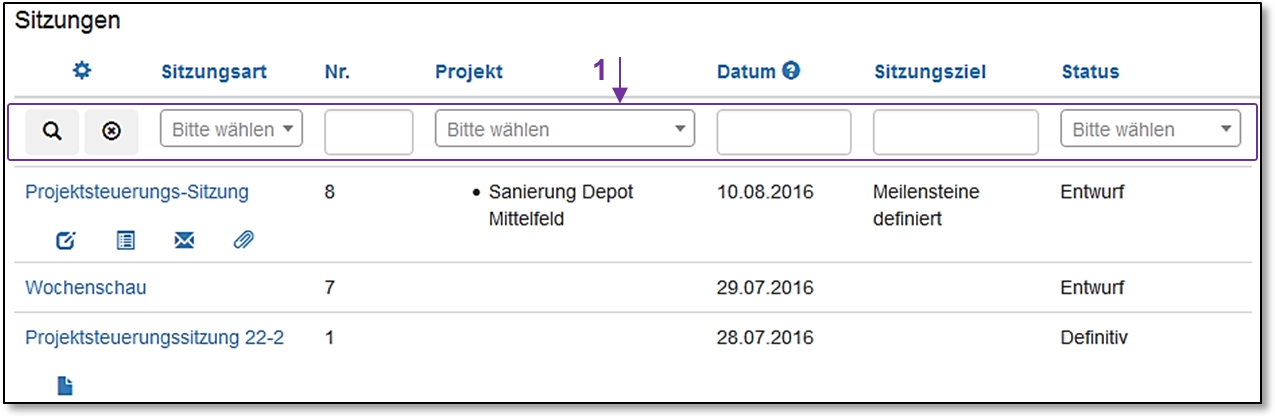
\includegraphics[width=1\linewidth]{../chapters/05_Sitzungswesen/pictures/5-2-1_SitzungenListe.jpg}}
\caption{Aperçu des séances recensées}
% \label{fig:speciation}
\end{figure}

\textbf{Fonction de filtrage}\col{(1)}

Utilisez la fonction de filtrage pour trouver la séance désirée. Remplissez les champs encadrés avec ce que sous savez / cherchez. Cliquez ensuite sur la loupe 
\includegraphics[height=12pt]{/Icons/Lupe_kl.jpg} ou appuyez la touche Entrée.

\vspace{\baselineskip}

Toutes les saisies qui correspondent aux critères de recherche sont affichées. Dans le champ 'Objectif de la séance' vous pouvez saisir n'importe quels mots-clé qui apparaît dans ce champ (vous n'avez pas besoin de mettre un caractère de remplacement * devant un mot).

\vspace{\baselineskip}

\textbf{Légende pour la modification de saisies de séances}

\vspace{\baselineskip}

\begin{tabular}{|c|p{14cm}|} %{cl}
\hline
\raisebox{-1\totalheight}{
\includegraphics[height=12pt]{/Icons/Blattsymbol.jpg}} & Le procès-verbal a été 'Archivé' et ne peut qu'être visualisé et non modifié \\
\hline
\raisebox{-.25\totalheight}{
\includegraphics[height=12pt]{/Icons/Bearbeiten.jpg}} & Modifier l'invitation à la séance, voir chapitre \ref{bkm:Ref434828480} \\
\hline
\raisebox{-.25\totalheight}{
\includegraphics[height=12pt]{/Icons/Kalenderimport.jpg}} & Importer l'invitation à la séance directement sous format .ics-file dans un calendrier Outlook \\
\hline
\raisebox{-.25\totalheight}{
\includegraphics[height=12pt]{/Icons/Listensymbol.jpg}} & Modifier le procès-verbal de la séance \\
\hline
\raisebox{-.25\totalheight}{
\includegraphics[height=12pt]{/Icons/Versandsymbol.jpg}} & Envoyer l'invitation à la séance avec ses pièces jointes correspondantes \\
\hline
\raisebox{-.25\totalheight}{
\includegraphics[height=12pt]{/Icons/Briefsymbol.jpg}} & Ouvrir l'invitation sous format PDF (pour envoi par e-mail ou par poste) \\
\hline
\raisebox{-.25\totalheight}{
\includegraphics[height=12pt]{/Icons/Bueroklammer.jpg}} & Des pièces jointes sont inclues dans cette invitation \\
\hline
\end{tabular}

\vspace{\baselineskip}

Repérez une séance dans la liste et cliquez sur le symbole 
\includegraphics[height=12pt]{/Icons/Listensymbol.jpg} à droite. Le mode 'Modifier procès-verbal de séance' s'affiche avec le masque pour saisir le procès-verbal de la séance. \\

\begin{figure}[H]
\vspace{-20pt}  
\center{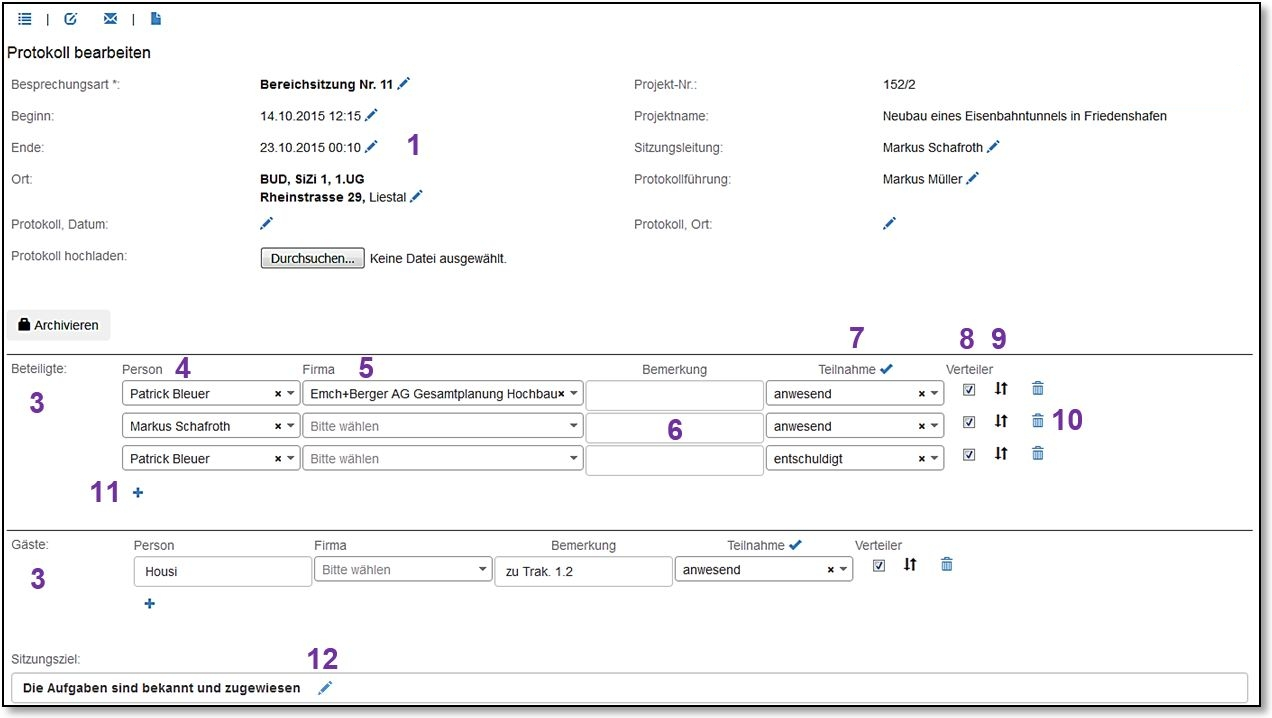
\includegraphics[width=1\linewidth]{../chapters/05_Sitzungswesen/pictures/5-2-1_ProtokollBearbeiten.jpg}}
\caption{Modifier un procès-verbal de séance}
% \label{fig:speciation}
\end{figure}

\begin{figure}[H]
\center{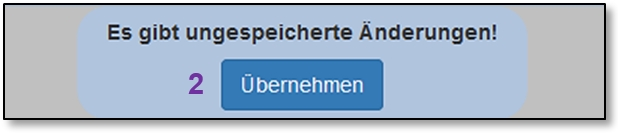
\includegraphics[width=0.4\linewidth]{../chapters/05_Sitzungswesen/pictures/5-2-1_Uebernehmen_top.jpg}}
% \caption{Das Menü in CUBE PA}
% \label{fig:speciation}
\end{figure}

\begin{itemize}
\item
Les champs type de séance, début, fin, lieu, numéro et nom de projet, directeur de séance et auteur du procès-verbal en-haut dans le masque sont automatiquement remplis avec les données de l'invitation. Pour modifier un de ces champs, cliquez sur le symbole de crayon qui se trouve à côté de chaque champ 
\includegraphics[height=12pt]{/Icons/Stift.jpg} \col{(1)} et modifiez la saisie. Le lieu et la date du procès-verbal ont chacun un champ : avec sélection calendrier pour la date et une liste de sélection pour le lieu. Cliquez sur le bouton 'Actualiser' \col{(2)} (en bas à gauche ou en haut au milieu) pour sauvegarder les modifications.
\item
Modifier les domaines 'Participants' et 'Invités' \col{(3)} fonctionne de la même manière que lors de la création de l'invitation à la séance. Cliquez sur le champ 'Personne' \col{(4)} ou 'Entreprise' \col{(5)} pour choisir un autre nom ou une autre entreprise de la liste de sélection. Dans le champ 'Remarques' \col{(6)} vous pouvez ajouter des remarques sous forme de texte libre, par exemple 'présent jusqu'à 9h'. Dans le champ 'Participation' \col{(7)} vous pouvez choisir entre 'Présent' et 'Excusé'. Cochez la case 'Distribution' \col{(8)} pour ajouter une personne à la liste de distribution. Utilisez le symbole de flèches verticales 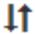
\includegraphics[height=12pt]{/Icons/VertPfeile.jpg} \col{(9)} pour modifier l'ordre des participants.
\item
Cliquez sur le symbole poubelle \includegraphics[height=12pt]{/Icons/Muelltonne.jpg} \col{(10)} pour supprimer un participant. Cliquez sur le signe plus (ajouter) \includegraphics[height=12pt]{/Icons/Pluszeichen.jpg} \col{(11)} pour en ajouter un.
\item
Les invités sont modifiés, ajoutés et supprimés de la même façon.
\item
L'objectif de la séance peut être modifié en cliquant sur le symbole crayon \includegraphics[height=12pt]{/Icons/Stift.jpg} \col{(12)} correspondant.
\item
Cliquez sur le bouton 'Actualiser' \col{(2)} pour sauvegarder vos changements.
\end{itemize}

Sous l'objectif de la séance, les points d'ordre du jour apparaissent.

\begin{figure}[H]
\center{\includegraphics[width=1\linewidth]{521_Traktanden.jpg}}
\caption{La liste des points d'ordre du jour}
% \label{fig:speciation}
\end{figure}

Dans cette section vous pouvez saisir le texte du procès-verbal, ainsi que les décisions et les affaires en suspens.

\begin{itemize}
\item
Vous pouvez modifier la liste de points d'ordre du jour comme vous l'avez déjà fait en créant l'invitation : Cliquez sur les signes plus (ajouter) \includegraphics[height=12pt]{/Icons/Pluszeichen.jpg} \col{(1)} pour ajouter un nouveau point, et sur le symbole poubelle \includegraphics[height=12pt]{/Icons/Muelltonne.jpg} \col{(2)} pour en supprimer un. Utilisez le symbole de flèches verticales \includegraphics[height=12pt]{/Icons/VertPfeile.jpg} \col{(3)} pour modifier l'ordre des points.
\item
Cliquez sur les flèches horizontales \includegraphics[height=12pt]{/Icons/Pfeil-links-rechts.jpg} \col{(4)} pour modifier la structure :

	\begin{itemize}
		\item
		La structure standard est 1, 2, 3 etc. \col{(a)}
		\item
		Cliquez une fois sur la flèche pointant vers la droite \includegraphics[height=12pt]{/Icons/Pfeil-rechts.jpg} \col{(b)} et la ligne sélectionnée est déplacée sous le point précédent, numéro 1, et prend le numéro 1.1 \col{(c)}.
		\item
		Si vous ne voulez pas une structure numérotée sous un point d'ordre du jour, mais simplement un nouveau paragraphe, cliquez à nouveau sur la flèche pointant vers la droite \includegraphics[height=12pt]{/Icons/Pfeil-rechts.jpg} \col{(d)} : La ligne n'est plus numérotée et un paragraphe normal est créé sous le numéro précédent \col{(e)}.
		\item
		Cliquez sur la flèche pointant vers la gauche \includegraphics[height=12pt]{/Icons/Pfeil-links.jpg} \col{(f)} pour annuler les changements.
	\end{itemize}
\end{itemize}

\begin{figure}[H]
\center{\includegraphics[width=1\linewidth]{521_Protokoll_ordnen.jpg}}
\caption{La structure du procès-verbal}
% \label{fig:speciation}
\end{figure}

Pour saisir le texte d'un point d'ordre du jour du procès-verbal, cliquez le symbole d'expansion \includegraphics[height=12pt]{/Icons/Aufklappen.jpg} \col{(5)} (un petit triangle dans un carré) à côté du titre du point d'ordre du jour. Un champ dans lequel vous pouvez saisir du texte libre pour ce point d'ordre du jour \col{(6)} s'affiche.

\vspace{\baselineskip}

Les quatre symboles sous le champ de texte ont les fonctionnalités suivantes :

\begin{figure}[H]
\center{\includegraphics[width=1\linewidth]{521_EntscheidSymbole.jpg}}
\caption{Options pour les décisions}
% \label{fig:speciation}
\end{figure}

\begin{itemize}
\item
Voulez-vous saisir une décision qui sera automatiquement recensée dans la liste de décisions ? Cliquez sur le symbole à gauche \includegraphics[height=12pt]{/Icons/Gutzeichen_Rahmen.jpg} \col{(a)} et une fenêtre s'ouvre, dans laquelle vous pouvez saisir la décision. Les champs 'Titre' \col{(1)} et 'Description' \col{(2)} sont des champs de texte libre. Le champ 'Projet / Sous-projet' \col{(3)} est une liste de sélection. Cliquez sur le bouton 'Créer' \col{(4)} pour sauvegarder la décision ou sur la croix \col{(6)} pour l'annuler.

\begin{figure}[H]
\center{\includegraphics[width=0.75\linewidth]{521_EntscheidHinzufuegen.jpg}}
\caption{Ajouter une décision}
% \label{fig:speciation}
\end{figure}

\end{itemize}

\begin{itemize}
\item
Voulez-vous saisir une affaire en suspens qui sera directement recensée dans la liste d'affaires en suspens ? Cliquez sur le deuxième symbole de gauche\includegraphics[height=12pt]{/Icons/Pfeil_aus_Box.jpg} \col{(b)} et une fenêtre s'ouvre, dans laquelle vous pouvez saisir l'affaire en suspens. Les champs 'Titre' \col{(1)} et 'Description' \col{(2)} sont des champs de texte libre. Le champ 'Délai' \col{(3)} est un calendrier à partir duquel la date peut être choisie. Les autres champs \col{(4)} sont des listes de sélection. Cliquez sur le bouton 'Créer' \col{(5)} pour sauvegarder l'affaire en suspens ou la croix \col{(6)} pour l'annuler.

\begin{figure}[H]
\center{\includegraphics[width=0.75\linewidth]{521_PendenzHinzufuegen.jpg}}
\caption{Ajouter une affaire en suspens}
% \label{fig:speciation}
\end{figure}

\end{itemize}

\begin{figure}[H]
\center{\includegraphics[width=1\linewidth]{521_EntscheidSymbole2.jpg}}
\caption{Transformer des points d'ordre du jour en décisions ou en affaires en suspens}
% \label{fig:speciation}
\end{figure}

\begin{itemize}
\item
Les décisions et les affaires en suspens sauvegardées apparaissent directement en-dessous du point d'ordre du jour correspondant.
\item
Si vous remarquez que le texte que vous venez d'écrire est en fait une décision, cliquez sur l'avant-dernier symbole à droite \includegraphics[height=12pt]{/Icons/Pfeil_Gutzeichen.jpg} \col{(c)}. Le texte apparaît dans une fenêtre dans laquelle vous pouvez compléter les détails de la décision et la sauvegarder. \textbf{Attention} : le texte est déplacé et non copié dans la fenêtre de la décision !
\item
Si vous remarquez que le texte que vous venez d'écrire est en fait une affaire en suspens, cliquez sur le dernier symbole à droite \includegraphics[height=12pt]{/Icons/Pfeil_Pfeil_aus_Box.jpg} \col{(d)}. Le texte apparaît dans une fenêtre dans laquelle vous pouvez compléter les détails de l'affaire en suspens et la sauvegarder. \textbf{Attention} : le texte est déplacé et non copié dans la fenêtre de l'affaire en suspens !
\end{itemize}

% \vspace{\baselineskip}

\textbf{Renseignement} : Il n'est pas nécessaire de saisir le texte du procès-verbal d'une manière parfaitement structurée dès le début. Copier-coller fonctionne comme dans Microsoft Word : sélectionnez le texte que vous aimeriez copier et faites un clic droit (menu contextuel) ou utiliserz les raccourcis clavier 'Ctrl+C' (copier), 'Ctrl+X' (couper) et 'Ctrl+V' (insérer). Vous pouvez par exemple saisir tout le texte sous le premier point d'ordre du jour et le répartir sur les autres points après la séance. Les décisions et les affaires en suspens peuvent également être ajoutées ultérieurement.

\vspace{\baselineskip}

\textbf{Formater le texte du procès-verbal :}

% \vspace{\baselineskip}

Dès que vous cliquez sur un champ de texte du procès-verbal, une bande avec des boutons pour le formatage \col{(1)} apparaît. Ces boutons fonctionnent comme les boutons correspondants dans Microsoft Word :

\begin{figure}[H]
\center{\includegraphics[width=1\linewidth]{521_TextFormatieren.jpg}}
\caption{Formater le texte}
% \label{fig:speciation}
\end{figure}

\begin{compactitem}
\item Gras : afficher le texte sélectionné en caractères gras
\item Italique : afficher le texte sélectionné en caractères italiques
\item Souligner : souligner le texte sélectionné
\item Couleur de fond : colorer le fond du texte sélectionné 
\item Exposant : mettre le texte sélectionné en exposant
\item Éliminer le formatage : enlever tous les formatages du texte sélectionné
\item Insérer de MS-Word : insérer un texte que vous avez sélectionné et copié dans 
Microsoft Word directement dans le champ de texte
\item Annuler : annule le dernier changement
\item Récupérer : récupère un changement annulé
\item Liste numérotée : transforme le lignes sélectionnées 
en liste numérotée
\item Liste : transforme le lignes sélectionnées 
en liste
\item Diminuer l'alinéa : déplacer le texte sélectionné vers la gauche
\item Augmenter l'alinéa : déplacer le texte sélectionné vers la droite
\item Insérer un tableau : insérer un tableau à la position actuelle du curseur.
Une fenêtre dns laquelle vous pouvez définir les paramètres pour votre tableau s'affiche.
Expérimentez avec les possibilités.
\end{compactitem}

\vspace{\baselineskip}

\begin{sloppypar}
Au côté droit des boutons pour le formatage se trouvent les boutons pour le mode révision. Cette fonction est expliquée plus tard dans le chapitre \ref{bkm:Ref434478117}.
\end{sloppypar}

\pagebreak
\subsubsection{Charger le procès-verbal en tant que document}

Préparez le procès-verbal comme d'habitude en tant que document, par exemple dans Microsoft Word, et le faites-le approuver par le reste des participants. Dès que vous avez une version définitive, générez un fichier PDF et chargez-le sur CUBE PA :

\vspace{\baselineskip}

\begin{wrapfigure}[7]{l}{6.5cm}   % [x] Wie manche Zeile soll sich um die Grafik "brechen"
  \vspace{-35pt}      % Grundwert war 20; mit 30 schön oben beim Text ausgerichtet
  \begin{center}
    \includegraphics[width=1\linewidth]{../chapters/05_Sitzungswesen/pictures/5-1_Menu_Sitzungswesen.jpg}
  \end{center}
  \vspace{-20pt}
  \caption{La Gestion de séances}
  \vspace{-10pt}
\end{wrapfigure}

Dans le menu principal à gauche, choisissez l'élément de menu 'Gestion de séances', puis le sous-élément 'Séances'. Vous êtes dirigé vers un aperçu de toutes les séances enregistrées dans CUBE PA, c'est-à-dire les séances pour lesquelles au moins une invitation a été créée. \newline

\vspace{6.5cm} 

Repérez une séance dans la liste et cliquez sur le symbole \includegraphics[height=12pt]{/Icons/Listensymbol.jpg} \col{(1)} à droite :

\begin{figure}[H]
\center{\includegraphics[width=1\linewidth]{../chapters/05_Sitzungswesen/pictures/5-2-2_Sitzungsuebersicht.jpg}}
\caption{Aperçu des séances recensées}
% \label{fig:speciation}
\end{figure}

\vspace{\baselineskip}

Le masque pour saisir le procès-verbal de la séance s'affiche :

\begin{figure}[H]
\center{\includegraphics[width=1\linewidth]{../chapters/05_Sitzungswesen/pictures/5-2-2_ProtokollErfassen.jpg}}
\caption{Saisir le procès-verbal}
% \label{fig:speciation}
\end{figure}

\textbf{Astuce :} Au lieu de cliquer sur 'Naviguer' sous 'Charger procès verbal' pour sélectionner le procès verbal, vous pouvez glisser-déposer le fichier directement sur le champ 'Naviguer'. Le procès verbal sera chargé et lié à l'invitation à la séance.

\vspace{\baselineskip}

\begin{itemize}
\item
Les champs type de séance, début, fin, lieu, numéro et nom de projet, directeur de séance et auteur du procès-verbal en-haut dans le masque sont automatiquement remplis avec les données de l'invitation. Pour modifier un de ces champs, cliquez sur le symbole de crayon qui se trouve à côté de chaque champ \includegraphics[height=12pt]{/Icons/Stift.jpg} \col{(1)} et modifiez la saisie. Le lieu et la date \col{(2)} du procès-verbal ont chacun un champ : avec sélection calendrier pour la date et une liste de sélection pour le lieu. Cliquez sur le bouton 'Actualiser' \col{(3)} (en bas à gauche ou en haut au milieu) pour sauvegarder les modifications. Il n'est pas nécessaire de remplir tous les champs. Remplissez au moins ceux qui permettent d'identifier la séance clairement.
\item
Cliquez sur 'Naviguer' \col{(4)} sous 'Charger procès-verbal' et choisissez le fichier PDF contenant le procès-verbal avec un double-clic. Ensuite cliquez sur 'Actualiser'. L'information 'Le procès-verbal est joint comme fichier' apparaît en rouge \col{(5)}, ce qui indique que le processus est terminé. Si vous avez chargé le mauvais document, vous pouvez le supprimer en cliquant sur le symbole poubelle. Un autre document pourra ensuite être chargé.
\end{itemize}

\vspace{\baselineskip}

\textbf{Attention :} Seuls les fichiers PDF sont acceptés. Si un document d'un autre type - par exemple un document Word - est chargé, ceci mène à un message d'erreur en l'ouvrant dans un PDF-reader.

\vspace{\baselineskip}

En chargeant le document, tous les utilisateurs CUBE PA peuvent lire le procès-verbal n'importe où et à tout moment, comme s'il avait été directement établi dans CUBE PA. Quand vous êtes sûr que le procès-verbal est complet et correct, cliquez sur le bouton 'Archiver' \col{(6)} et confirmez le message \col{(7)}. CUBE PA fixe l'état de la séance comme 'Définitive' et le procès-verbal ne peut plus être modifié, ni un autre procès-verbal chargé.

\begin{figure}[H]
\center{\includegraphics[width=0.5\linewidth]{522_Archivieren.jpg}}
\caption{Archiver le procès-verbal}
% \label{fig:speciation}
\end{figure}

\subsubsection{Ajouter des pièces jointes à un procès-verbal}

La section pour charger des pièces jointes se trouve sous la section pour saisir le texte du procès-verbal.

\begin{figure}[H]
\center{\includegraphics[width=1\linewidth]{../chapters/05_Sitzungswesen/pictures/5-2-3_ProtokollBeilagen.jpg}}
\caption{Télécharger des pièce jointes au provès-verbal}
% \label{fig:speciation}
\end{figure}

Le procédé principal est semblable à celui pour charger un procès-verbal :

\begin{itemize}
\item
Cliquez sur le signe plus (ajouter) \includegraphics[height=12pt]{/Icons/Pluszeichen.jpg} \col{(1)} pour ajouter une pièce jointe.
\item
Vous pouvez saisir le titre, la version et la description de la pièce jointe \col{(2)}.
\item
Sous 'Charger nouveau fichier' \col{(3)}, cliquez 'Naviguer' et choisissez le fichier désiré avec un double-clic. Si vous avez téléchargé le mauvais document, chargez simplement un nouveau et cliquez sur 'Actualiser'.
\item
Vous pouvez changer l'ordre des pièces jointes par glisser-déposer en utilisant le symbole des flèches verticales \includegraphics[height=12pt]{/Icons/VertPfeile.jpg} \col{(4)} ou supprimer une pièce jointe en cliquant sur le symbole de poubelle \includegraphics[height=12pt]{/Icons/Muelltonne.jpg} \col{(5)}.
\end{itemize}

\vspace{\baselineskip}

\textbf{Astuce} : Au lieu de cliquer sur 'Naviguer' sous 'Charger procès verbal' pour sélectionner le document, vous pouvez glisser-déposer le fichier directement sur le champ 'Naviguer'. Le fichier sera chargé et lié à l'invitation à la séance.

\vspace{\baselineskip}

\textbf{Remarque} : Les pièces jointes ne sont pas automatiquement jointes à la version PDF du procès-verbal. Le seul but de leur chargement est de les rendre accessibles aux autres utilisateurs de CUBE PA.

\subsection{Faire contrôler un procès-verbal et l'archiver}
\label{bkm:Ref434478117}
Si vous avez créé un procès-verbal dans CUBE PA, les participants peuvent le vérifier et le corriger. Le procès-verbal peut ensuite être finalisé.

\vspace{\baselineskip}

Pour vérifier et corriger un procès-verbal, choisissez l'élément de menu 'Gestion de séances' dans le menu principal à gauche, puis le sous-élément 'Séances'. Une liste apparaît avec toutes les séances recensés dans CUBE PA. Une liste similaire apparaît également dans l'aperçu personnel. Tant que le procès-verbal est en état 'Projet', des changements peuvent y être apportés. Cliquez alors sur le symbole \includegraphics[height=12pt]{/Icons/Listensymbol.jpg} \col{(1)} à gauche.

\begin{figure}[H]
\center{\includegraphics[width=1\linewidth]{../chapters/05_Sitzungswesen/pictures/5-2-2_Sitzungsuebersicht.jpg}}
\caption{Aperçu des séances}
% \label{fig:speciation}
\end{figure}

\vspace{\baselineskip}

Vous pouvez maintenant modifier tous les champs. Si vous voulez un suivi de qui a apporté des chanhements, utilisez le mode révision. Celui fonctionne de la manière suivante :

\vspace{\baselineskip}

Dès que vous cliquez dans un champ de texte du procès-verbal, une bande avec des boutons apparaît \col{(1)}. Ces boutons fonctionnent comme les boutons correspondants dans Microsoft Word. Le bloc de boutons à droite gère le mode révision :

\begin{figure}[H]
\center{\includegraphics[width=1\linewidth]{53_Ueberarbeitungsmodus.jpg}}
\caption{Activer le mode révision}
% \label{fig:speciation}
\end{figure}

\begin{itemize}
\item
Activer et désactiver le mode révision \col{(2)} : Cliquez sur ce bouton pour activer et désactiver le mode révision. Après l'avoir activé, les changements que vous faites sont marqués \col{(3)} et CUBE PA documente qui a fait ces changements et quand \col{(4)}.
\end{itemize}

\begin{figure}[H]
\center{\includegraphics[width=1\linewidth]{53_UeberarbeitungsmodusReferenz.jpg}}
\caption{Référence de révision}
% \label{fig:speciation}
\end{figure}

Les autres boutons sont importants pour la finalisation du procès-verbal.

\begin{figure}[H]
\center{\includegraphics[width=.75\linewidth]{53_Formatierungen.jpg}}
\caption{Finalisation du procès-verbal}
% \label{fig:speciation}
\end{figure}

\begin{itemize}
\item
Accepter tous les changements \col{(5)} : tous les changements dans un champ de texte sont acceptés.
\item
Accepter le changement \col{(6)} : le changement sélectionné est accepté.
\item
Rejeter tous les changements \col{(7)} : tous les changements dans un champ de texte sont rejetés.
\item
Rejeter le changement \col{(8)} : le changement sélectionné est rejeté.
\end{itemize}

\vspace{\baselineskip}

Avant d'archiver le procès-verbal, vous pouvez aussi en générer un fichier PDF pour le lire. Sous 'Modifier procès-verbal de séance' en haut à gauche se trouve un groupe de quatre symboles. Cliquez sur le symbole de feuille \includegraphics[height=12pt]{/Icons/Blattsymbol.jpg} \col{(1)} tout à droite pour en générer un PDF.

\begin{figure}[H]
\center{\includegraphics[width=1\linewidth]{53_ProtokollArchivieren.jpg}}
\caption{Archiver le procès-verbal}
% \label{fig:speciation}
\end{figure}

Si vous êtes sûr que le procès-verbal est correct cliquez sur le bouton 'Archiver' \col{(2)} et confirmez le message \col{(3)}. CUBE PA fixe l'état de cette séance à 'Définitive' et le procès-verbal ne peut plus être modifié.

\subsection{Créer des affaires en suspens}

Vous pouvez aussi créer des affaires en suspens indépendamment d'un procès-verbal. Dans le menu principal à gauche, choisissez l'élément de menu 'Gestion de séances' puis le sous-élément 'Affaires en suspens'. Vous êtes dirigé vers la liste d'affaires en suspens.

\vspace{\baselineskip}

Cliquez sur le signe plus (ajouter) \includegraphics[height=12pt]{/Icons/Plussymbol.jpg} \col{(1)} en haut à gauche et la fenêtre 'Créer affaire en suspens' apparaît avec le masque de saisie d'une nouvelle affaire en suspens.

\begin{figure}[H]
\center{\includegraphics[width=1\linewidth]{../chapters/05_Sitzungswesen/pictures/5-4_Pendenzen.jpg}}
\caption{Saisir une affaire en suspens}
% \label{fig:speciation}
\end{figure}

\textbf{Légende des couleurs :}

\begin{tabular}{c p{14cm} l} %{cl}
\includegraphics[height=12pt]{/Icons/PunktGruen.jpg} & Le délai de l'affaire en suspens est encore 'loin' \\
\includegraphics[height=12pt]{/Icons/PunktGelb.jpg} & Le délai de l'affaire en suspens approche \\
\includegraphics[height=12pt]{/Icons/PunktRot.jpg} & L'affaire en suspens est en retard \\
\end{tabular}

\vspace{\baselineskip}

L'utilisation du marqueur jaune dépend de la durée totale de l'affaire en suspens (date de création jusqu'à date d'échéance).

\begin{figure}[H]
\center{\includegraphics[width=1\linewidth]{54_PendenzenErfassen.jpg}}
\caption{Saisir une affaire en suspens}
% \label{fig:speciation}
\end{figure}

Remplissez les champs.

\begin{itemize}
\item
Les champs 'Titre' \col{(1)} et 'Description' \col{(2)} sont des champs de texte libre.
\item
Le champ 'Délai' \col{(3)} est choisi d'un calendrier alors que tous les autres champs \col{(4)} sont des listes de sélection. Le champ 'État' est par défaut fixé à 'en suspens'. Ceci est l'état normal pour une affaire en suspens qui vient d'être créée.
\end{itemize}
Cliquez sur 'Créer' \col{(5)} pour ajouter l'affaire en suspens à la liste des affaires en suspens.

\subsection{Chercher, lire et modifier des affaires en suspens}
Pendant le déroulement du projet il se peut que la révision d'affaires en suspens devienne nécessaire, par exemple pour les marquer comme terminées, pour modifier leurs délais ou pour préciser leurs contenus. Pour ce faire, il faut chercher et modifier une affaire en suspens dans la liste d'affaire en suspens.

\vspace{\baselineskip}

Pour chercher une ou plusieurs affaires en suspens, choisissez l'élément de menu 'Gestion de séances' du menu, puis le sous-élément 'Affaires en suspens'. La liste des affaires en suspens s'affiche :

\begin{figure}[H]
\center{\includegraphics[width=1\linewidth]{../chapters/05_Sitzungswesen/pictures/5-5_PendenzenUebersicht.jpg}}
\caption{Chercher une affaire en suspens}
% \label{fig:speciation}
\end{figure}

Vous pouvez maintenant chercher une affaire en suspens optiquement en parcourant la liste ou bien vous pouvez utiliser la fonction de filtrage. Pour parcourir la liste, utilisez la pagination en bas de la page pour avancer / reculer dans la liste ou aller à une page spécifique.

\begin{figure}[H]
\center{\includegraphics[width=.25\linewidth]{/Icons/SeitenBlaettern.jpg}}
% \label{fig:speciation}
\end{figure}

Vous pouvez utiliser les champs de recherche dans la première ligne de la liste des affaires en suspens pour filtrer la liste. Les champs 'Titre' et 'Description' sont des champs de texte libre. Les champs 'Type de séance', 'Projet / Sous-projet', 'Responsable', 'Collaboration', 'Comité responsable' et 'État' sont des listes de sélection. Vous pouvez saisir un numéro de séance dans le champ 'ID' et utiliser le calendrier pour remplir le champ 'Délai'. Quand vous avez choisi vos données de filtrage, cliquez sur le symbole de loupe \includegraphics[height=12pt]{/Icons/Lupe_kl.jpg} \col{(1)} à gauche ou appuyez la touche Entrée pour voir la liste filtrée.

\begin{figure}[H]
\center{\includegraphics[width=1\linewidth]{../chapters/05_Sitzungswesen/pictures/5-5_PendenzenFelderBearbeiten.jpg}}
\caption{Modifier des affaires en suspens}
% \label{fig:speciation}
\end{figure}

Le symbole de feuille \includegraphics[height=12pt]{/Icons/Blattsymbol_s.jpg} \col{(2)} en haut à gauche vous permet de générer un fichier PDF de la liste des affaires en suspens.

\vspace{\baselineskip}

Si vous voulez retourner à la liste des affaires en suspens entière, effacez les critères de filtrage. Dans les champs avec une liste de sélection ceci se fait en cliquant sur la petite croix \col{(3)} à droite dans le champ. Pour les autres champs, sélectionnez le texte et effacez le contenu. Après avoir effacé toutes les données, cliquez à nouveau sur le symbole de loupe \includegraphics[height=12pt]{/Icons/Lupe_kl.jpg} \col{(1)} ou appuyez la touche Entrée.

\begin{center}
\includegraphics[height=14pt]{55_PendenzenFeldLoeschen.jpg}
\end{center}

Il existe deux possibilités pour modifier une affaire en suspens. Vous pouvez faire les modifications directement dans la liste en cliquant sur le symbole de crayon \includegraphics[height=12pt]{/Icons/Stift.jpg} \col{(4)} à gauche d'un champ, en changeant le contenu du champ, puis en cliquant le symbole de coche \includegraphics[height=12pt]{/Icons/Gutzeichen.jpg} \col{(5)} sous le champ pour sauvegarder le changement. L'état de l'affaire en suspens se modifie par la liste de sélection \col{(6)}. La deuxième option est de cliquer sur le symbole de modification \includegraphics[height=12pt]{/Icons/Bearbeiten.jpg} \col{(7)} à gauche d'une affaire en suspens. La fenêtre 'Modifier affaire en suspens' \col{(8)} s'affiche et vous pouvez alors changer le contenu des champs dans le masque puis cliquer sur 'Actualiser' pour sauvegarder les changements. Cliquez ensuite sur le symbole de liste \includegraphics[height=12pt]{/Icons/Listensymbol_zurueck.jpg} \col{(9)} pour retournez à la liste des affaires en suspens. La sélection déjà filtrée reste active.


\begin{figure}[H]
\center{\includegraphics[width=1\linewidth]{55_PendenzenBearbeiten.jpg}}
\caption{Modifier une affaire en suspens}
% \label{fig:speciation}
\end{figure}

L'état d'une affaire en suspens peut prendre les valeurs suivantes (selon la configuration du projet) :

\begin{compactitem}
\item
En suspens : L'affaire en suspens a été ouverte mais pas encore traitée. Cette valeur est automatiquement fixée à la création de l'affaire en suspens (valeur par défaut).
\item
En traitement : Le responsable a fait son travail et changé l'état à 'En traitement'.
\item
Terminée : La séance interne du directeur général confirme que l'affaire en suspens est terminée.
\item
Conclusion confirmée : Au type de séance dans laquelle l'affaire en suspens a été crée, 
on confirme que celle-ci est bien terminée.
\end{compactitem}

\subsection{Chercher et lire des décisions}

Pour lire une décision, choisissez l'élément de menu 'Gestion de séances' du menu principal à gauche, puis le sous-élément 'Décisions'. La liste des décisions s'affiche. Vous pouvez la filtrer et la parcourir comme la liste des affaires en suspens. Vous pouvez aussi générer un fichier PDF de cette liste. Cependant, vous ne pouvez pas ajouter une nouvelle décision, ni en modifier une . Les décisions peuvent uniquement être crées ou modifiées dans le cadre d'un procès-verbal.

\subsection{Lire des procès-verbaux}

Pour lire un procès-verbal choisissez l'élément de menu 'Gestion de séances' dans le menu principal à gauche puis le sous-élément 'Séances'. La liste des séances s'affiche.

\begin{figure}[H]
\center{\includegraphics[width=1\linewidth]{../chapters/05_Sitzungswesen/pictures/5-7_ProtkolleLesen.jpg}}
\caption{Lire un procès-verbal}
% \label{fig:speciation}
\end{figure}

Vous pouvez parcourir cette liste et la filtrer comme la liste des affaires en suspens.

\begin{itemize}
\item
Si le procès-verbal est à l'état 'Définitif' (le bouton 'archiver' a été cliqué), cliquez sur le symbole de feuille \includegraphics[height=12pt]{/Icons/Blattsymbol.jpg} \col{(1)} à gauche de la séance correspondante (cliquez sur la séance désirée pour afficher les options). Ceci génère un fichier PDF du procès-verbal ou télécharge un document de procès-verbal qui a été chargé comme fichier PDF.
\item
Si le procès-verbal est à l'état 'Brouillon', cliquez sur le symbole \includegraphics[height=12pt]{/Icons/Listensymbol.jpg} \col{(2)} à gauche de la séance correspondante pour ouvrir la fenêtre 'Modifier procès-verbal', dans laquelle vous pouvez lire le contenu du procès-verbal. Ceci ne fonctionne que si le procès-verbal est recensé directement dans CUBE PA. Vous n'avez que l'accès à un procès-verbal chargé si le bouton 'Archiver' a été cliqué et que le procès-verbal est à l'état 'Définitif'.
\end{itemize}
